\chapter{Robot Operating System}

\textbf{Author: Lukas Leskovar} 

This chapters objective is to describe the basic concepts of the Robot Operating System (ROS) utilized by Autumn. The ROS despite its name is a meta-operating system or middleware providing the utility and services often found in robotics frameworks. It enables the composition of distributed systems by utilizing publisher-subscriber communication between different programs of such systems. Furthermore ROS provides a comprehensive set of tools enabling the compilation, operation as well as testing, visualization and debugging of robotic systems. With its vast amount of libraries and huge open-source community providing useful functionality ROS facilitates the development of robotic applications without having to reimplement standardized technology. \footcite{openSourceRoboticsFoundationDefinitionNodate}


\section{Conceptual Overview}
The Robot Operating System can be divided into three conceptual levels each contributing a integral part to the utility of ROS. These different levels are described in the following sections. \footcite{openSourceRoboticsFoundationConceptsNodate}

\subsubsection{File System}
The File System Level mainly provides constraints and best practices for creating and structuring packages and their components. 
ROS provides appropriate tools to facilitate file-system operations with and within packages.
%operations such as searching for packages or file within packages
%With appropriate tooling the ROS facilitates file-system operations within packages, messages or topics. 

\subsubsection{Computational Graph}
The Computational Graph provides crucial functionality to ROS as it refers to the peer-to-peer mesh network of processes (nodes) each providing data to be utilized within the graph by publishing and subscribing to topics.
The concepts and technologies powering the computational graph are described in later in this chapter.

\subsubsection{Community}
The Community preserves the usability of ROS as new and useful packages and tools are created as well as existing functionality is being maintained.

\section{Naming}
To aid the organization of programs, processes as well as resources ROS provides two naming schemes that are described in the following sections. \citereset\footcite{openSourceRoboticsFoundationConceptsNodate}

\subsubsection{Graph Resource Names}
Graph Resource Names utilize a hierarchical structure to organize nodes, services, topics or anything else within the computational graph. ROS defines four different types of names:
%\begin{itemize}
%	\item base names - Are resolved in the same fashion as relative names
%	\item relative names - Are resolved relatively starting by the nodes name
%	\item global names - Begin with a / and are considered fully resolved
%	\item private names - Begin with a $\tilde{ }$ and convert the nodes name into a namespace
%\end{itemize}

\subsubsection{Package Resource Names}
Package Resource Names aim to facilitate the search process of resources at File System Level. These names usually consist of the packages name as well as the path to the desired resource within the package. 
%Examples for such Names are:
%\begin{itemize}
%	\item 
%\end{itemize}

\section{Packages}
Software in ROS is organized in packages containing nodes, libraries or any other piece of software providing functionality.

%noch ein bisschen trennen (atomic build item, ...)
%der absatz gefällt mir nicht, eigentlich gehört da nur die atomicity hin
%In order to maintain reusability, atomicity and easy decoupling of functionality packages aim to be as slim as possible by implementing only a limited-set of features. This means that each package is develop to focus on one task alone and work together with other packages to deliver utility as a connected system.
Since packages are the atomic unit of build and release they aim to be a slim as possible my implementing only a limited set of features. 
In other words packages should be implemented to provide minimal usability without being too large-scaled.\footcite{openSourceRoboticsFoundationPackageNodate} This means that each package is developed to work together with other packages to deliver utility as a connected system.  

At file-system level packages simply refer to directories. While most subfolders and files within a package depend on its purpose, every package has to contain a package.xml and a CMakeLists.txt providing meta and build information.
Packages can be build by utilizing rosbuild or catkin. \footcite{openSourceRoboticsFoundationBuildNodate}

\subsubsection{Metapackages} 
Metapackages are specialized packages only containing a package.xml that logically links multiple related packages.\footcite{openSourceRoboticsFoundationMetapackageNodate}
They can be used to conveniently install a group of packages simultaneously. %naja ned so wirklich



\section{Nodes}
The goal of ROS is to promote code reusability and decoupling of functionality to aid the versatility and usability of the system. 
Following this guideline every robotic system utilizing ROS consists of a fine-grained graph of processes called nodes. Each node provides computation on a single feature utilizing a ROS client library to communicate with others over a mesh-like peer-to-peer network. \footcite{openSourceRoboticsFoundationNodesNodate}

Exemplary for such as system would be one node running a LiDAR sensor, one responsible for localization, one performing motion planning, one controlling motor drivers and motors as well as one node running the robots main control loop.

This architecture allows for a much more fault safe and less complex applications in comparison to monolithic systems. \footcite[Page 94]{stephensBeginning2015}
This means that development and debugging are facilitated since errors can be contained within a singular slim node rather than a larger program. 

Each node has a node type consisting of the package name it is located and as well as the nodes executable. 



\section{Communication}

\subsection{Messages}
Messages are the medium of communication used in topics or services to transport data between nodes. 
%They are used to send data between nodes over topics or through services. 

\subsubsection{Message Description}
A message is a simple data structure consisting of multiple type fields. These fields can be primitives, arrays, custom types as well as other message types. \footcite{openSourceRoboticsFoundationMessagesNodate}

The message description language can be used to structure custom messages in
\textit{.msg} files contained in the \textit{msg} directory of a package.

\subsubsection{Message Types}
Message types refer to package resource names consisting of the packages name as well as the name of the messages \textit{.msg} file.


\subsection{Topics}
The core component of communication in ROS are topics. They are unidirectional message streams enabling data transmission by utilizing the publisher-subscriber model 
 %utilizing the publisher-subscriber model to establish data transmission in a many-to-many relationship.
Furthermore the decoupling of functionality is facilitated by anonymously connecting nodes as producer and consumer of data. This means neither publisher nor subscriber of the topic need to know each other. 
While ROS does not limit the amount of publishers and subscribers connected to a topic, it strictly enforces the usage of the exact message type specified for the topics communication to work properly.

\subsection{Services}
The communication architecture in ROS utilizing the publisher-subscriber model is advantageous in most use-cases, however most distributed systems require remote procedure calls (RPC) which are not supported by default.

With RPCs a client sends a request to a server specifying the procedure to be called and its parameters. While the server executes the procedure the client awaits a reply. Once the procedures results are computed and sent to the client its workflow can be resumed.\footcite[Page 3]{rfc1831}

Services enable communication over RPC by defining a pair of messages, one for requests and one for replies. Such service can then be attached to a node and called by a client using the service name. \footcite{openSourceRoboticsFoundationServicesNodate}




\section{Master}
One of the most important components of ROS is the Master. It tracks publishers and subscribers of topics as well as services and provides registration as well as name resolution to nodes. This means whenever a node wants to publish or subscribe to a specific topic or service it contacts the master first using XML-RPC. When a topic has at leat one subscriber and publisher the Master negotiates between the nodes so a peer-to-peer connection can be established using a Slave API provided by the nodes XML-RPC Server.\footcite{openSourceRoboticsFoundationMasterNodate} A simplified version of this procedure can be seen in Fig. \ref{fig:ros_master_reg}

Besides registration and name resolution, the ROS Master also provides a Parameter Server used for globally storing static system parameters.\footcite{openSourceRoboticsFoundationParameterServerNodate}
\begin{figure}[]
	\centering
	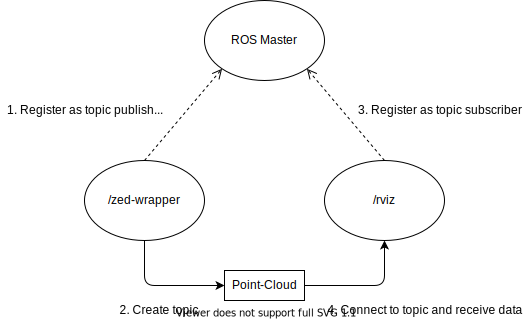
\includegraphics[width=0.8\linewidth]{img/ros_master_registration}
	\caption{Diagram of the topic registration process in ROS at which the publishing node registers its topic before the subscriber tells the master its interest in the point-cloud topic. However a node can be registered as a subscriber to a specific topic without the topic existing yet.}
		\label{fig:ros_master_reg}
\end{figure}



\section{Transform Library}
A complex robotic system consists of multiple parts such as sensors, cameras, manipulators, etc. which are each represented as a coordinate frame, where each frame is connected to another frame using joints. When trying to move a specific part or coordinate frame, not only the transform of that single frame but the composite transform of each frame in relation to the target has to be calculated. This is especially important when moving a robotic arm based on sensor readings. In this example a transform between the position of the sensor and the arm needs to be calculated so the motion performed by the arm the motion perceived by the sensor match.
Using the ROS Transform Library (tf) these complex calculations can be facilitated. To this end tf keeps track of each coordinate frame in a acyclic relationship tree where tf broadcasters then publish relative pose information and listeners query transforms between two coordinate frames. 
Because not all pose information in a robotic system is instantly accessible, the tf saves this information for each frame over time. This means that transforms can be queried not just spacially but also temporally.



\section{Simulation}



\subsection{URDF}



\subsection{Gazebo Simulator}



\filbreak